\documentclass[main.tex]{subfiles}
\begin{document}

\section*{Tue Dec 17 2019}

\begin{figure}[ht]
    \centering
    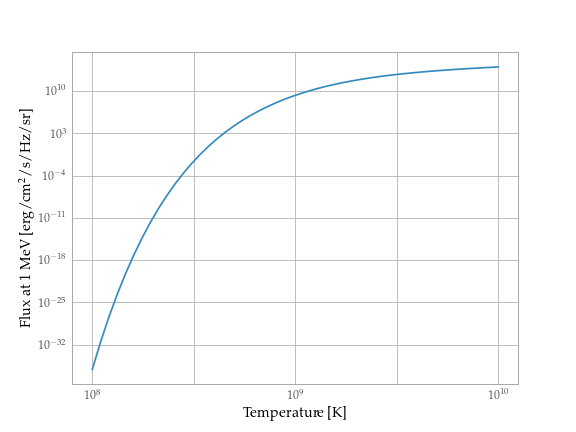
\includegraphics[width=\textwidth]{figures/flux_1_MeV.png}
    \caption{Flux at \SI{1}{MeV} for a blackbody with varying temperature \(T\).}
    \label{fig:flux-1-MeV}
\end{figure}

The number of pulsation instabilties decreases as the He core mass increases. After \(60 M_{\odot}\) only one pulsation is needed in order to blow off the whole core. 

People generally focus on low metallicity, very massive stars. For example, they are found in the Magellanic clouds. 

Many factors affect the growth of the oxygen core: 
\begin{enumerate}
    \item \(\ce{^{12}C}(\alpha , \gamma ) \ce{^{16}O}\) rate;
    \item convection reduces the minimum mass for a PCSN;
    \item rotation-induced chemical mixing: this reduces the minimum stellar mass needed in order to have a PCSN;
    \item rotation decreases the binding energy: it increases the maximum mass needed in order to have a PCSN.
\end{enumerate}

Plots of the nuclear, binding and kinetic energies are useful to understand the process. 

The nuclear front crosses the various layers of the star. 
If we increase the initial mass of the star, the amount of Nickel produced increases a lot. 

We can plot the production factor of various nuclides relative to the solar rate of production: as the isotope number \(Z\) varies: we plot \(\log (\text{prod} / \text{solar prod})\). We see a zig-zag pattern: a large difference between even and odd nuclides. Even ones are produced more. 

Nickel is important because of the decay chain \(\ce{Ni} \rightarrow \ce{Co} \rightarrow \ce{Fe}\), which could explain the shape of the decaying light curve of the supernova. 

Referring to PCSNe: how much to they contribute to the chemical composition of galaxies? 
We can plot the metal yield multiplied by the probability to have a star of that mass (which is roughly \(\varphi (M) \sim M^{-2.5}\)) as the mass of the star varies. We include Core Collapse SNe (with \(M < 50 M_{\odot}\)), then there is a BH region, and then we have PISNe from \(120 M_{\odot}< M < 260 M_{\odot}\), then BHs again. 

Partial test on the 14th of January.

\end{document}